\documentclass[12pt, titlepage]{article}

\usepackage{pdflscape}
\usepackage{fullpage}
\usepackage[round]{natbib}
\usepackage{multirow}
\usepackage{booktabs}
\usepackage{tabularx}
\usepackage{graphicx}
\usepackage{float}
\usepackage{hyperref}
\hypersetup{
    colorlinks,
    citecolor=blue,
    filecolor=black,
    linkcolor=red,
    urlcolor=blue
}

%% Comments

\usepackage{color}

\newif\ifcomments\commentstrue %displays comments
%\newif\ifcomments\commentsfalse %so that comments do not display

\ifcomments
\newcommand{\authornote}[3]{\textcolor{#1}{[#3 ---#2]}}
\newcommand{\todo}[1]{\textcolor{red}{[TODO: #1]}}
\else
\newcommand{\authornote}[3]{}
\newcommand{\todo}[1]{}
\fi

\newcommand{\wss}[1]{\authornote{blue}{SS}{#1}} 
\newcommand{\plt}[1]{\authornote{magenta}{TPLT}{#1}} %For explanation of the template
\newcommand{\an}[1]{\authornote{cyan}{Author}{#1}}

%% Common Parts

\newcommand{\progname}{MTOBridge} % PUT YOUR PROGRAM NAME HERE
\newcommand{\authname}{Team 15, Alpha Software Solutions
\\ Badawy, Adham
\\ Yazdinia, Pedram
\\ Jandric, David
\\ Vakili, Farzad
\\ Vezina, Victor
\\ Chiu, Darren} % AUTHOR NAMES                  

\usepackage{hyperref}
    \hypersetup{colorlinks=true, linkcolor=blue, citecolor=blue, filecolor=blue,
                urlcolor=blue, unicode=false}
    \urlstyle{same}


\newcounter{acnum}
\newcommand{\actheacnum}{AC\theacnum}
\newcommand{\acref}[1]{AC\ref{#1}}

\newcounter{ucnum}
\newcommand{\uctheucnum}{UC\theucnum}
\newcommand{\uref}[1]{UC\ref{#1}}

\newcounter{mnum}
\newcommand{\mthemnum}{M\themnum}
\newcommand{\mref}[1]{M\ref{#1}}

\begin{document}

\title{System Design for \progname{}} 
\author{\authname}
\date{\today}

\maketitle

\pagenumbering{roman}

\section{Revision History}

\begin{tabularx}{\textwidth}{p{2.5cm}p{3.5cm}X}
\toprule {\bf Date} & {\bf Developer(s)} & {\bf Change}\\
\midrule
15/01/2023 & Farzad & Initial Draft\\
17/01/2023 & Victor & Added Timeline and Protocol Design\\
18/01/2023 & Adham & Added Reflection\\
18/01/2023 & Darren & Added Reflection\\
18/01/2023 & Pedram & Added Reflection\\
18/01/2023 & David & Added Reflection\\
18/01/2023 & Victor & Added Reflection\\
18/01/2023 & Farzad & Added Reflection\\
\bottomrule
\end{tabularx}

\newpage

\section{Reference Material}

This section records information for easy reference.

\subsection{Abbreviations and Acronyms}

\renewcommand{\arraystretch}{1.2}
\begin{tabular}{l l} 
  \toprule		
  \textbf{symbol} & \textbf{description}\\
  \midrule 
  \progname & This is the name of the program being designed\\
  \bottomrule
\end{tabular}\\

\newpage

\tableofcontents

\newpage

\listoftables

\listoffigures

\newpage

\pagenumbering{arabic}

\section{Introduction}
The following is a high level system design document for the MTOBridge software, a program for load rating bridges experiencing strain caused by self driving truck platoons. For more information on this software, you can consult the following documents as needed:\\
\href{../../SRS/SRS.pdf}{Link to SRS}\\
\href{../../HazardAnalysis/HazardAnalysis.pdf}{Link to HA}\\
\href{../../VnVPlan/VnVPlan.pdf}{Link to V\&V}\\
\href{../../Design/SoftArchitecture/MG.pdf}{Link to MG}\\
\href{../../Design/SystDesign/SystDes.pdf}{Link to MIS}

\section{Purpose}
This document is intended to provide a high-level view of the design decisions made with regards to the user interface component of the MTOBridge software, along with a planned timeline of implementation.

\section{Scope}
Note that this document, as well as all others written by this team, will focus purely on the visualization and user interface component of MTOBridge, ignoring the backend MATLAB solvers as this component will not be designed by this team, nor does this team have any hand in that design. A simple diagram outlining the system boundaries can be found below.
\begin{figure}[H]
  \centering
  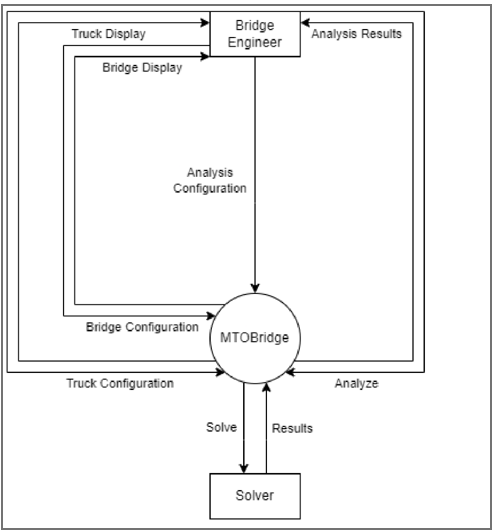
\includegraphics[]{../images/system-boundaries.PNG}
  \caption{System Boundaries Diagram}
  \label{fig:system-boundaries-diagram}
\end{figure}

\section{Project Overview}

\subsection{Normal Behaviour}
Assuming everything goes smoothly, the most general user scenario for MTOBridge is as follows:
\begin{enumerate}
\item A user launches the program
\item They set up/load a truck platoon configuration
    \begin{itemize}
        \item [2a.] They may choose to save their configuration for later
    \end{itemize}
\item They set up/load a bridge configuration
    \begin{itemize}
        \item [3a.] They may choose to save their configuration for later
    \end{itemize}
\item They set up/load a solver configuration
    \begin{itemize}
        \item [4a.] They may choose to save their configuration for later
    \end{itemize}
\item They run the calculations
\item A visualization of the results is presented to them
\item The output report is created and shown to them
\item The out report is saved to the file system
    \begin{itemize}
        \item [8a.] They may choose to return to step 1
    \end{itemize}
\item They exit the program
\end{enumerate}

\subsection{Undesired Event Handling}
As this is a user interface, robustness and reliability are of the utmost importance for a good user experience. Crashes, slowdowns, or hangs as a result of unexpected events will be highly detrimental to the quality of the program. With this in mind, the plan is to attempt to foresee and catch as many different types of errors as possible, and otherwise allow the program to fail in a palatable way. For example, if during step 4 the user inputs an invalid bridge configuration (i.e choosing “swaws” as the length of their bridge), the program will be set up to prompt them to enter another length, as their current one is invalid and it needs to be a number between x and y, say.
Another consideration is to design the program in such a manner so as to limit the possibility of undesired events occurring, by removing user freedom. For example, only allowing users to drag a slider from x to y meters to determine the length of their bridge rather than having them type it in, or some other form of input where the range of inputs can be controlled. This can make the program feel constrained, but also create a safer runtime where the user is not given enough rope to hang themselves.
Which of these undesired event handling techniques is applied will depend on the context, something like user input is simple and its errors are able to be caught well enough that the first method seems feasible. However, the amount of interaction with the visualization/animation of the calculation results available to the user is a much less discrete design space, and therefore might have to be limited using the second method. The choice of method and its application will be refined through testing, both for robustness and quality of life.

\subsection{Component Diagram}
N/A as there are no hardware or electrical components to this project

\newpage
\subsection{Connection Between Requirements and Design} 
\begin{table}[hp]
\centering
\caption{Connection Between Requirements and Design}
\label{TblRequirementsDesign}
\begin{tabular}{|p{0.2\textwidth}|p{0.8\textwidth}|}
\hline
Decisions & Requirement \\
\hline
Concurrency & NFR.9: UI elements react promptly\\ & NFR.10 UI will not be unreasonably slow.\\
\hline
MVC architecture & NFR.13: The product shall be easily maintainable.\\ & NFR.14: The program should be able to be easily translated into other languages. \\ & NFR.3: The product will appear correctly on different display resolutions.\\
\hline
Local File system & SR-8: The system must automatically save to a file.\\ & SR-3: The system must produce a log of function calls made to MATLAB.\\ & The log will include timestamps along with software environment information\\ & such as the current input.\\
\hline
\end{tabular}
\end{table}
Following concurrency best practices and its design implications ensures that the UI thread will never get stuck. Therefore, it can remain responsive and reacts promptly.\\\\
Incorporating the MVC architecture enables the separation of presentation components from the core logic. Firstly, this allows for a flexible presentation since different view modes can be “plugged” and “unplugged”. Secondly, taking advantage of such a feature makes altering the front-end source code more convenient because of it’s low coupling with other components.\\\\
Since the number of automatic saves is high, it’s wise to have a local data storage. Moreover, in order to prevent the automatic saving from taking a lot of space thus decreasing it’s value, a simple file system (vs a database) can be created where automatic saves are stored with the same filename overwriting the previous auto-saves. However, custom saves with a unique name given by the user will remain intact.  



\section{System Variables}

\subsection{Monitored Variables}
N/A
\subsection{Controlled Variables}
N/A
\subsection{Constants Variables}
N/A
\section{User Interfaces}
\begin{figure}[H]
  \centering
  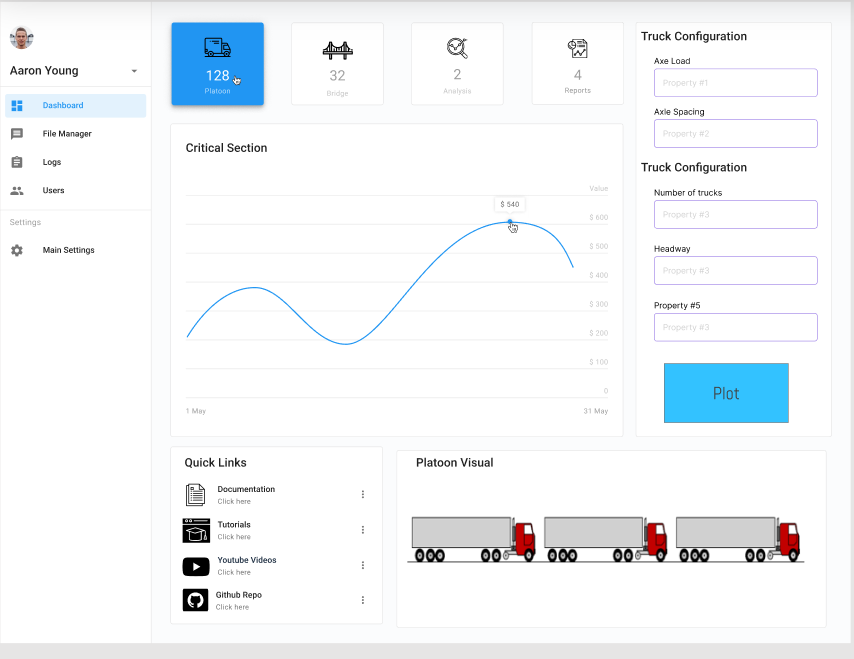
\includegraphics[width=1\textwidth]{../images/Userinterface-Platoon.PNG}
  \caption{User interface Platoon Diagram}
  \label{fig:userinterface-platoon-diagram}
\end{figure}
The screen where the user inputs information related to the truck configuration including the axle load, axle spacing, number of trucks and headway. A visual feedback of the inputted information is given at the bottom of the page to the user for confirmation. The effects of the specified platoon configuration to the critical/concerned section is displayed real-time as a graph in the middle of the screen. \\\\
\begin{figure}[H]
  \centering
  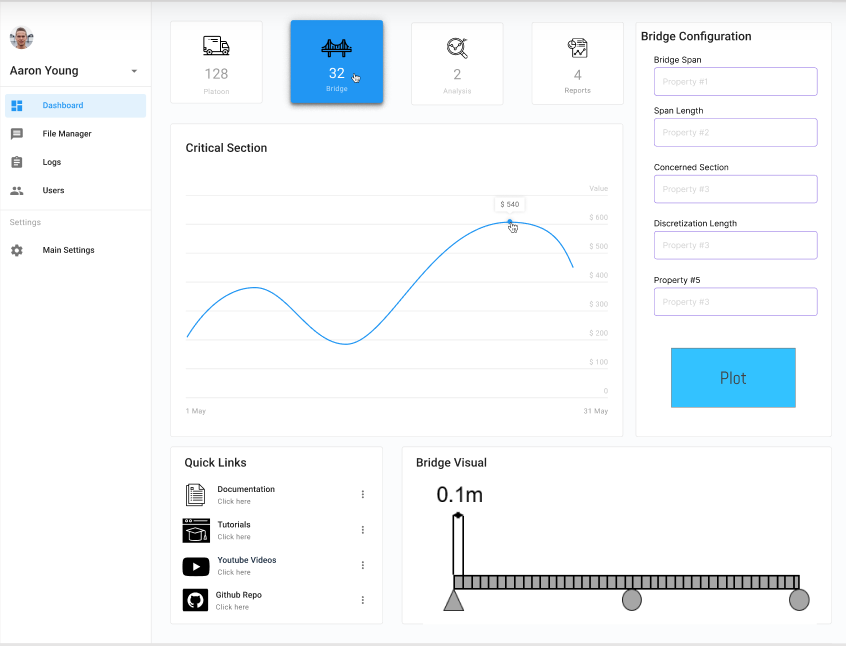
\includegraphics[width=1\textwidth]{../images/Userinterface-Bridge.PNG}
  \caption{User interface Bridge Diagram}
  \label{fig:userinterface-bridge-diagram}
\end{figure}
The screen where the user inputs information related to the Bridge configuration including the bridge span, span length, section of concern and the discretization length. A visual feedback of the inputted information is given at the bottom of the page to the user for confirmation. The effects of the specified bridge configuration to the critical/concerned section is displayed real-time as a graph in the middle of the screen.\\\\
\begin{figure}[H]
  \centering
  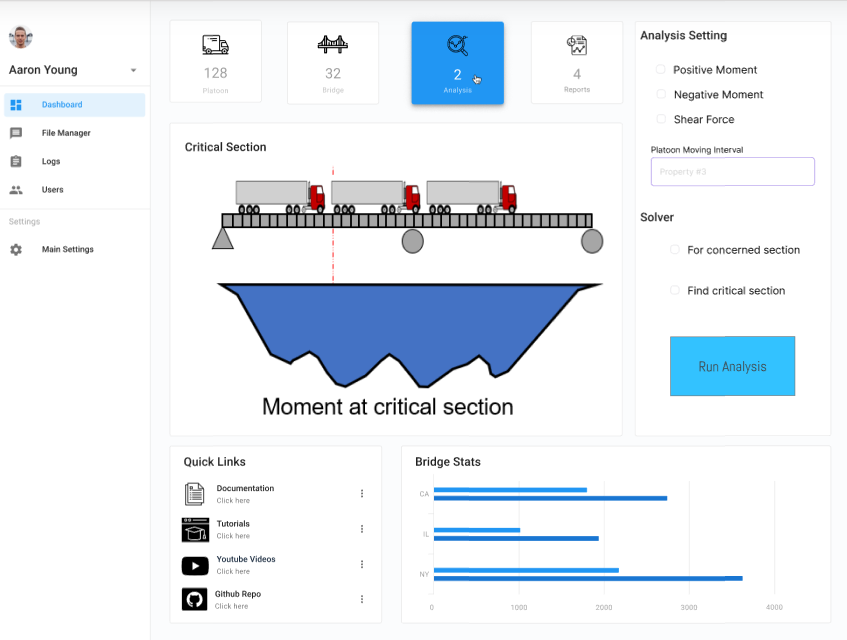
\includegraphics[width=1\textwidth]{../images/Userinterface-Analysis.PNG}
  \caption{User interface Analysis Diagram}
  \label{fig:userinterface-analysis-diagram}
\end{figure}
The screen where the user determines the Analysis setting as well as the section to be analyzed.Users can observe and verify the result of all of their customizations at bottom right corner of the page.\\\\
\begin{figure}[H]
  \centering
  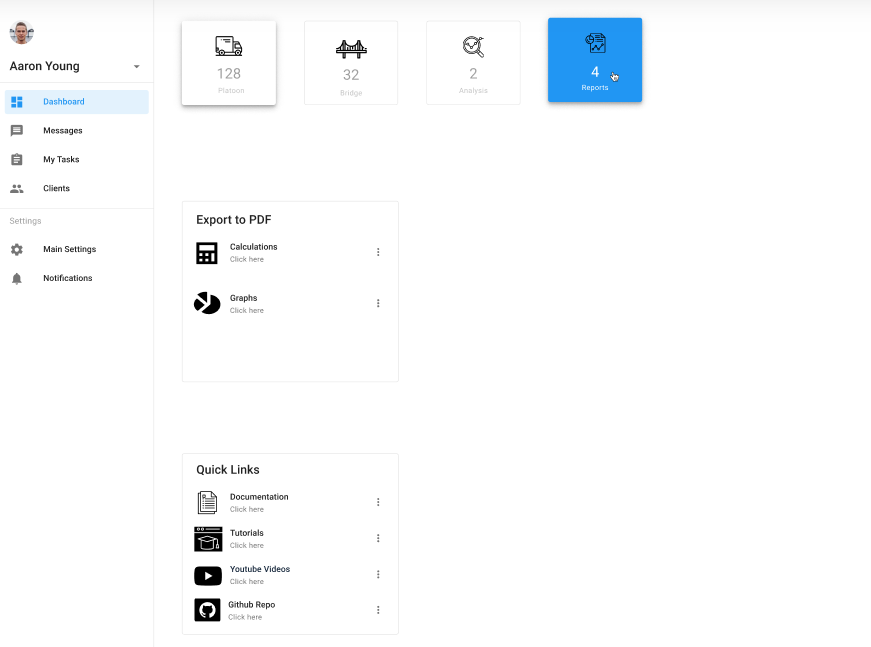
\includegraphics[width=1\textwidth]{../images/Userinterface-Report.PNG}
  \caption{User interface Report Diagram}
  \label{fig:userinterface-report-diagram}
\end{figure}
The screen where the calculations done by the solver and the outputted graphs can be exported to PDF.

\section{Design of Hardware}
N/A

\section{Design of Electrical Components}
N/A

\section{Design of Communication Protocols}

The only communication protocol used by the program is when it communicates with the MATLAB script. This actually uses two protocols: the method names and parameters defined in the MATLAB code, and the functionality implemented by the OS that allows our program to call the MATLAB script. Neither of these communication protocols has been designed by the project team.


\section{Timeline}

\begin{figure}[H]
  \centering
  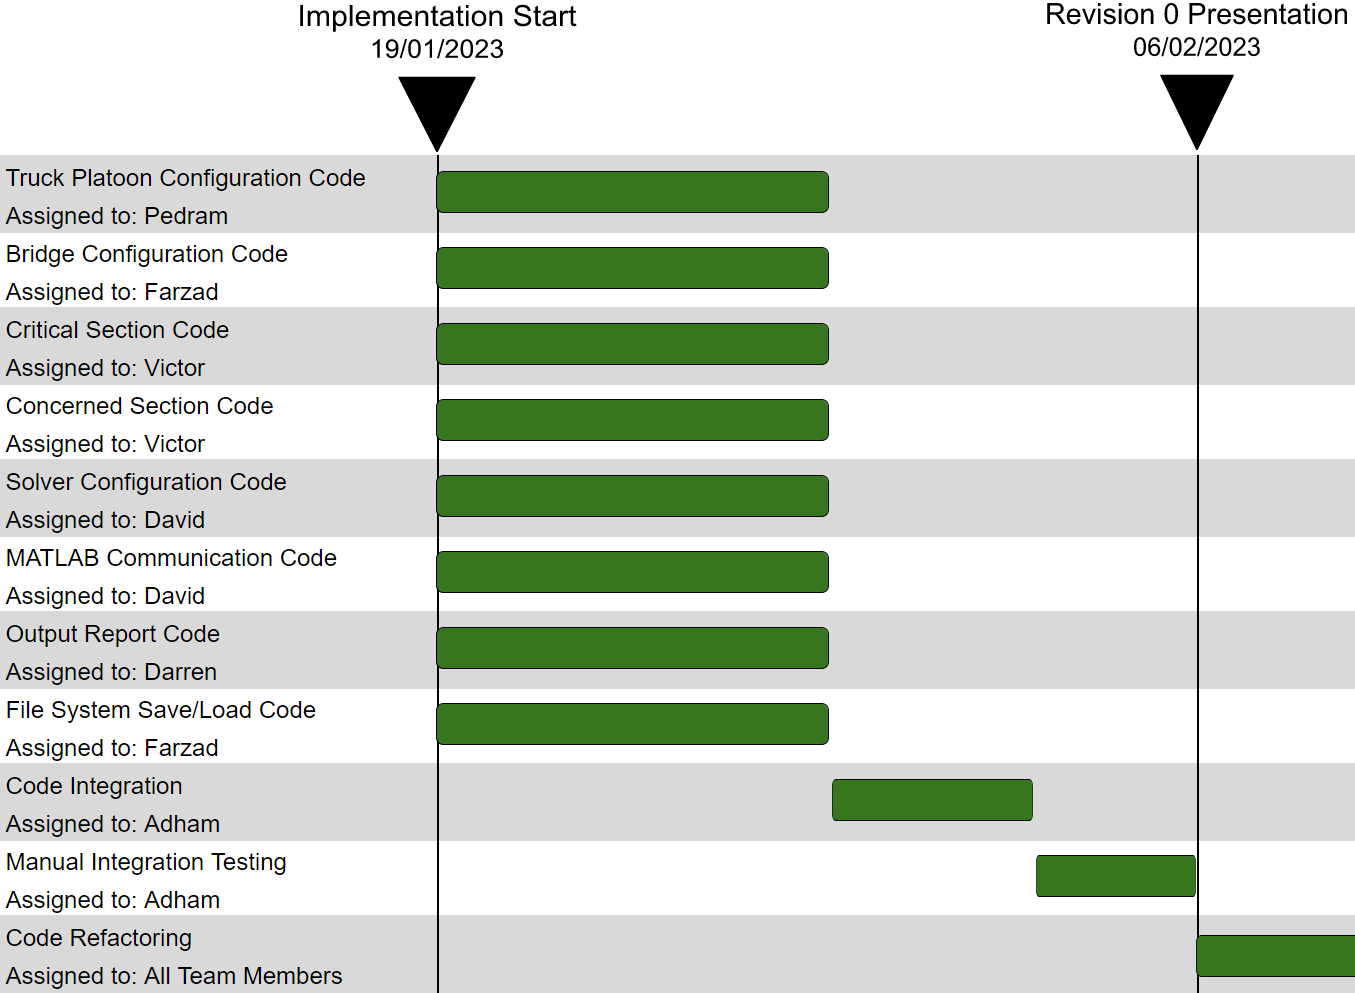
\includegraphics[scale=0.7]{../images/Timeline1.PNG}
  \caption{Project Timeline Section 1}
  \label{fig:timeline1}
\end{figure}

\begin{landscape}
\newpage

\begin{figure}[H]
  \centering
  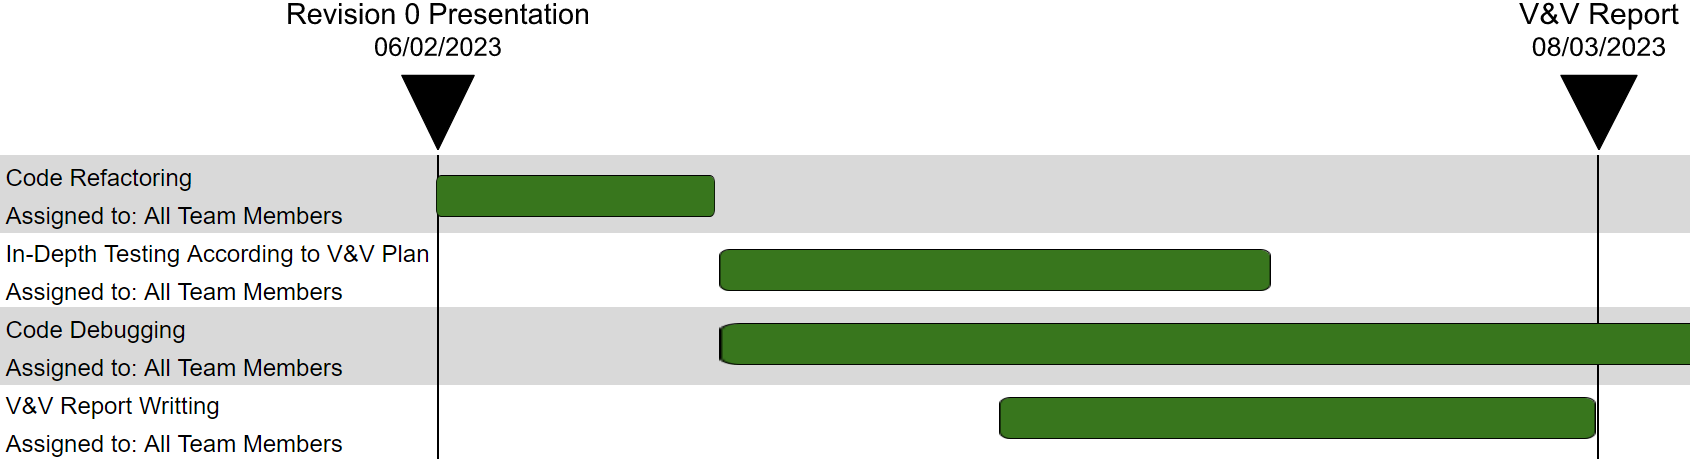
\includegraphics[scale=0.65]{../images/Timeline2.PNG}
  \caption{Project Timeline Section 2}
  \label{fig:timeline2}
\end{figure}

\begin{figure}[H]
  \centering
  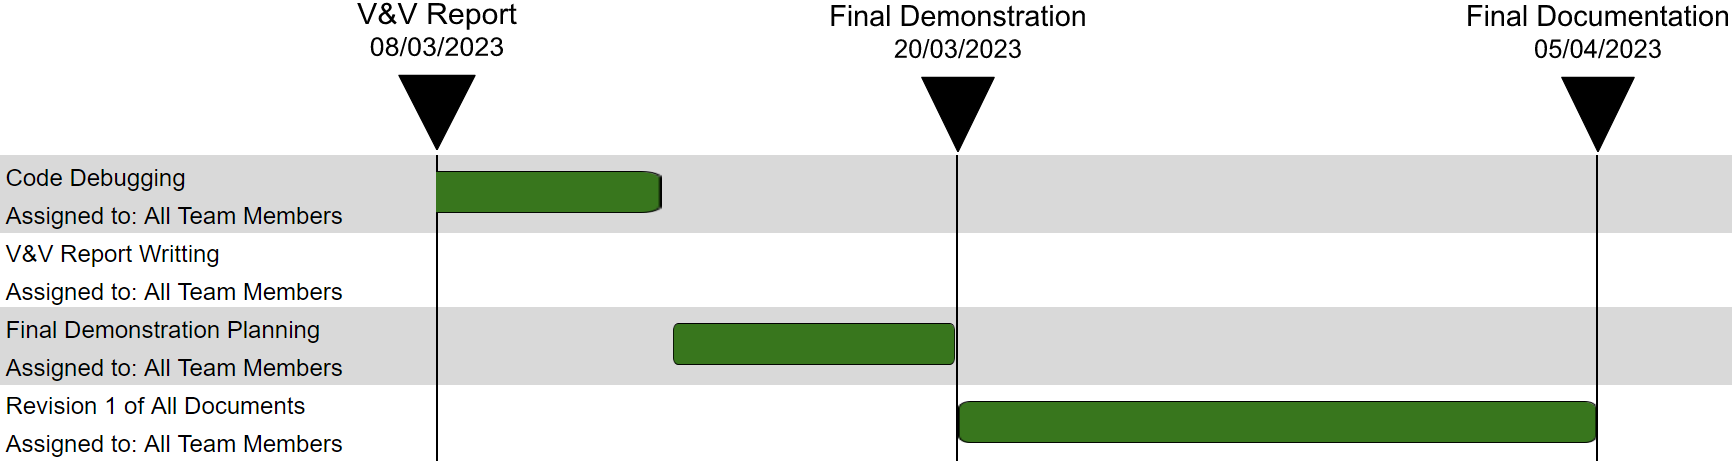
\includegraphics[scale=0.65]{../images/Timeline3.PNG}
  \caption{Project Timeline Section 3}
  \label{fig:timeline3}
\end{figure}

\end{landscape}

% \bibliographystyle {plainnat}
% \bibliography{../../../refs/References}

\newpage{}

\appendix

\section{Interface}

N/A

\section{Mechanical Hardware}
N/A
\section{Electrical Components}
N/A
\section{Communication Protocols}
N/A
\section{Reflection}

The information in this section will be used to evaluate the team members on the
graduate attribute of Problem Analysis and Design.  Please answer the following questions:

\begin{enumerate}
  \item What are the limitations of your solution?  Put another way, given
  unlimited resources, what could you do to make the project better? (LO\_ProbSolutions)
  \item Give a brief overview of other design solutions you considered.  What
  are the benefits and tradeoffs of those other designs compared with the chosen
  design?  From all the potential options, why did you select documented design?
  (LO\_Explores)
\end{enumerate}

\noindent\textbf{Adham}\\
I think the main aspect of the design that might be limited by time/resources is the presentation of the calculation results. In the worst case it may end up as just a 2D
representation or graph, when ideally we would want a 3D fully animated visual of the platoon as it travels across the bridge and the effects it has over the course of its
trip.\\

I think the main point of discussion as far as how to design the system was the level of modularity involved. As it stands, the project currently has 26 anticipated changes
corresponding 1 to 1 to 26 modules. over the course of the design process this ballooned as high as 30+ and some suggested designs shrank it down to closer to 10. We decided
to err more on the side of highly atomic modules in the end, for clarity and easy of understanding in the documentation, but still combined some modules that were extremely
trivial to avoid committing too dogmatically to a design principle even when it could be hurtful in practice.\\\\

\noindent\textbf{Darren}\\
Given time, could look at further configurability of platoons, e.g. accounting for trucks of different lengths, models, or wheel counts. Also for the animation to be a more 
faithful representation to better reflect the forces at play, such as alter the colors of the bridge display to reflect the stress on any given point.\\

Considered documenting further detail on subjects such as file I/O and graphics rendering. A generic visualizer module defining the exact nature of displaying 
a graphic to the screen was discussed to rigorously detail the design. We determined it was more important to focus efforts on the design of the system itself and the 
interaction of its parts rather than these modules to avoid reinventing the wheel.\\\\

\noindent\textbf{Victor}\\
I think one of the biggest limitations of our current design is the bridge input, as it allows for very little customization. That is, with more time we could implement a 
system that would allow the user to run calculations on more types and variations of bridges than the current design allows for.\\

We had considered designing our system so that it strictly followed the Model-View-Controller architectural pattern. While MVC would ease development and improve
maintainability, we decided that strictly following it would limit our design freedom too much. We decided to use our current design as it follows some of the same patterns,
allowing us to take advantage of many of the pros of MVC, while also giving us more flexibility.\\\\

\noindent\textbf{David}\\
I think, as Darren mentioned, the configurability of the truck platoon and the bridge could be enhanced greatly. For 
the bridge configurability, allowing for a larger number of bridge sections, defining bridge materials and section 
geometry could also be implemented. We could also enhance the way reports can be used, since they are essentially just
a text file, where it could be made into a format that accepts pictures (or maybe it creates the report in pdf form).\\

The calculation call module was one that we considered different solutions for. A design solution to this was to have
many external access programs, all of which would be a single call to the matlab engine. This would make the module
simpler, because it would avoid all the conditional logic. However, we decided against this because it would've just
shifted the responsibility to the users of this module. We instead decided to only have a single external access
program, with a unified input and output, and it's up to the other modules to decide how to use that output.\\\\

\noindent\textbf{Pedram}\\
With dozens of different Civil Engineering applications in the market, there is the opportunity to work on connecting our application with other platforms. This can be as simple as Import and Export functionalities or even adding our application as a plugin to their frameworks. The application, in theory, should also be capable of a cloud deployment where people can access through a webapp.\\

Creating an intuitive yet detailed UI with lots of options proved to be a main design challenge. The team debated on various layouts featuring design elements from animations, forms, tabs, and dynamic graphing. Members favored creating the UI from scratch as opposed to using partial templates to achieve specific functionalities enabled through a unique set of interactions between the graphs and the animations across all tabs. \\\\

\noindent\textbf{Farzad}\\
I think one of the biggest limitations of our project is the lack of drawing ability. This feature can enable a user to sketch a custom bridge and proceed with the analysis. Therefore, given unlimited developers as well as time incorporating such feature would significantly increase the value of the program by making it more flexible.\\

To accomodate for information saving the desicion between incorporting a relational databse to the overall architecture or using a simple filesystem was one of the points of discussion. The Team Decided that A file system is a better suit as the complexity that accompanies setting up a database doesn't outweight it's benefits. A local storage system that can easly be overwritten (Filesystem) would be a good solution to satisfy our Requirements.\\\\
\end{document}